
\section{Evaluation Results}
\subsection{Experimental Setup}

We evaluate the fusion optimization and kernel generation mechanisms on three modern image recognition tasks with transformers: DETR, SETR, and ViT. %Table xxx and Table xxx summarize workload characteristics.
We use PyTorch 1.7.1, cuDNN V7.6.5, CUDA 10.0, NVIDIA driver 460.67, and adopt TensorRT V7.0.0.11 and TVM 0.8.dev0, as well as the TensorRT version as baselines for our performance comparison study. All evaluation results are collected on a NVIDIA GeForce RTX 2080Ti GPU. \\
\textbf{Workflow.}The pipeline of our workflow can be summarized in the following two patterns: 1) For high-performance computing library TensorRT, we first use pytorch framwork to build transformer models 
with different paramemters, and then use the onnx export interface to export the pytorch model to onnx format. In order to avoid some redundant operators caused by conversion, we use onnx-simplifier to simplify the onnx model, and then convert it into an executable engine defined in TensorRT environment;
2) In terms of the compilation flow Ansor and AutoGTCO, we first convert the transformer model into torchscript format, and then use the pytorch interface defined in Relay to read the torchscript model. Finally, the corresponding tensor programs are generated by TVM code generation for the different subgraphs.

% We compare Automatic-E2EF against the state-of-art search frameworks and hardware-specific manual libraries. In the meantime, we evaluate the search
% efficiency of each module designed in Automatic-E2EF. 



% \subsection{Graph Fusion Analysis}

% \subsection{Kernel tunning Analysis}


\subsection{Comparsion of different Deep Learning Frameworks}
\textbf{Baselines and Configurations.} We first compare the inference performance among different compiler and neural network frameworks with batch size one on encoder in DETR-ResNet-50 model. 
There are three baselines: PyTorch JIT compiler, TensorRT, and Ansor. PyTorch JIT is a just-in-time compiler in pytorch, which is a way to create serializable and optimizable models from PyTorch code to a production environment where python
programs may be disadvantageous for performance and multi-threading reasons. TensorRT uses rule-based way to optimize the computation graph and the vender-provided library cuDNN for operator optimization. Ansor search the tensor program schedule for each kernel automatically. \\
\textbf{Results.} Table xxx shows that AutoGTCO consistently outperforms all three baselines on the different size of encoder for DETR-ResNet-50 model. AutoGTCD can achieve 
xxx to xxx speedup comparing to the state-of-the-art framework PyTorch JIT, TensorRT, and Ansor. Comparing with the rule-based optimization in Ansor, table xxx shows that AutoGTCD can generate suitable optimized subgraphs, and the weight of each subgraph is different from that of Ansor, which will help
to get a better schedule for tensor programs during the tuning process. In table xxx, \textbf{n} means the number of subgraphs in each part (such as encoder, decoder, transformer). The first number in square brackets indicates the number of times the subgraph needs to be tuned and the second number represents the number of subgraphs, which are both descirbed in subgraph scheduler section. The measurement trails is the auto-tuning time for the computation graph, which is described in performance tuner section. We can find that AutoGTCD takes less time to converage than Ansor.\\


\subsection{Subgraph Benchmark}
\textbf{Baselines and Configurations.} We perform the subgraph benchmark on three common subgraphs in DETR-ResNet-50 model: MHA, Encoder, and Decoder. The \textbf{MHA} is a subgraph consisting of \textbf{h} attention heads in parallel to attend to different learned projections of a sequence. Encoder and Decoder are both introduced in the background section. We use the same set of baseline framworks and run three benchmark on a NVIDIA GeForce RTX 2080Ti GPU.\\
\textbf{Results.} Figure \ref{fig:fig8} shows that AutoGTCD outperforms PyTorch JIT on the Encoder and Decoder by xxx speedup. 
For high-performance computing library TensorRT, AutoGTCD can achieve xxx speedup on MHA, Encoder, and Decoder.
For the compiler based search algorithm, AutoGTCD can achieve xxx speedup on MHA, Encoder, and Decoder.
It can prove that AutoGTCD can generate efficient tensor programs for these subgraphs on NVIDIA GPU platform.
% to attend to different learned projections of a sequence.
% {\color{red} multi-head attention, encoder and decoder}

% We perform the subgraph benchmark on two three subgraphs in tranformer. The multi-head attenion (mha) is a subgraph consisting of \textbf{h} attention heads in parallel
% to attend to different learned projections of a sequence. The \textit{encoder} is a subgraph consisting of \textbf{n} identical layers. Each layer has two sub-layers. The first is a mha mechanism, and the second is a simple,
% positionwise fully connected feed-forward network. The \textit{decoder} is a subgraph consisting of \textbf{n} identical layers. It inserts a third sub-layer, which performs multi-head attention over the output of 
% the encoder layer. We select three different shape configurations which corresponds to the image recognition benchmarks and two batch sizes, run auto-tuning with up to xxx
% measurement trails per test case, and report the normalized performance. In the meantime, we use the same set of paramters on the baseline framework. \\
% Figure xxx shows that our dynamic programming operator fusion technqiue outperforms manual libraries (tensorrt) and other search frameworks (ansor )by xxx.

\begin{figure}[htbp]
    \centering
    % 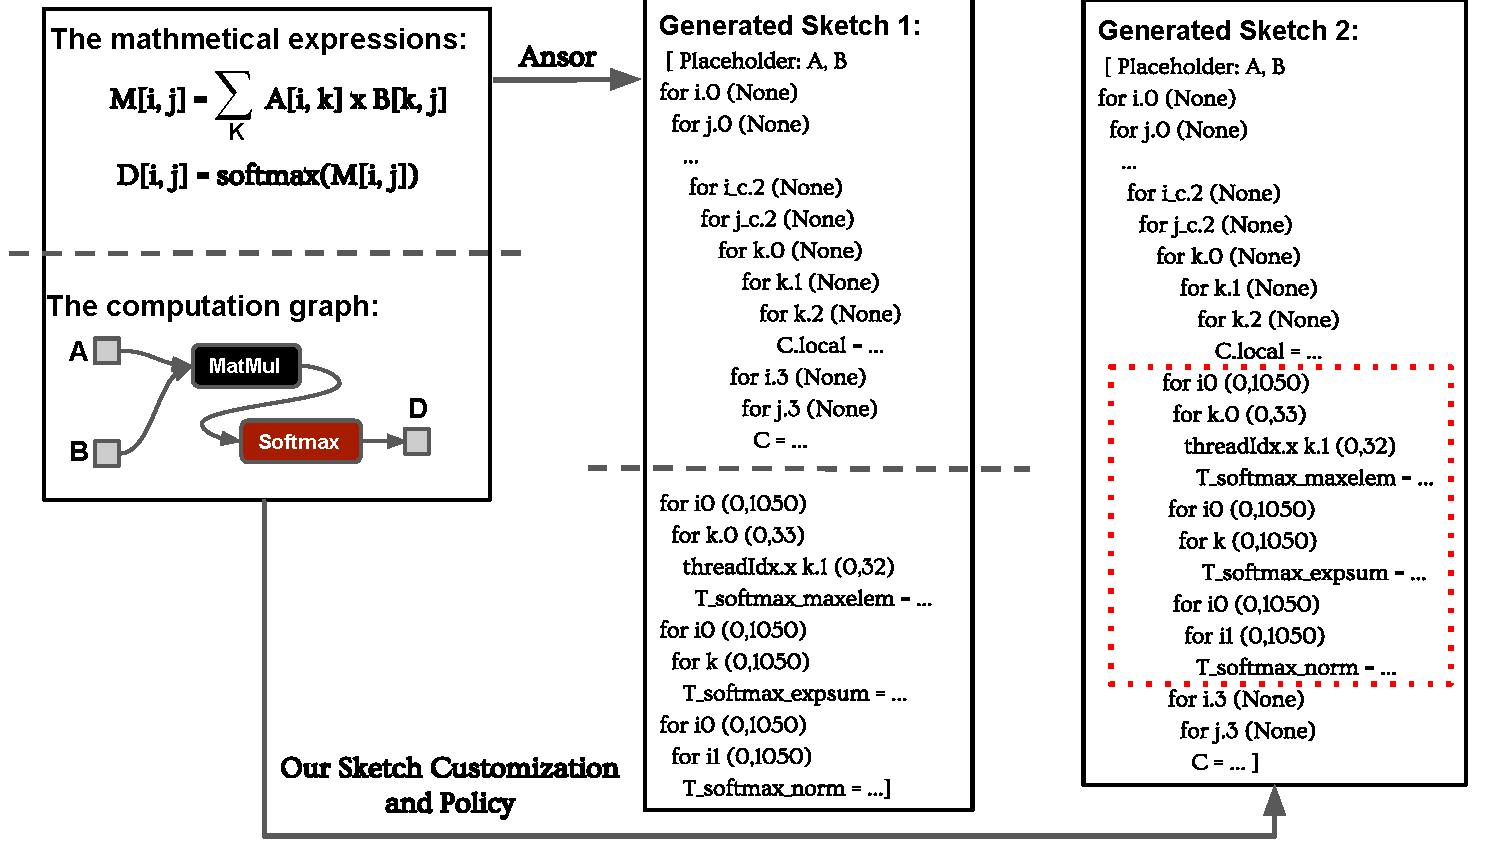
\includegraphics[width=10cm]{figs/fig4}
    % \hspace{1in}
    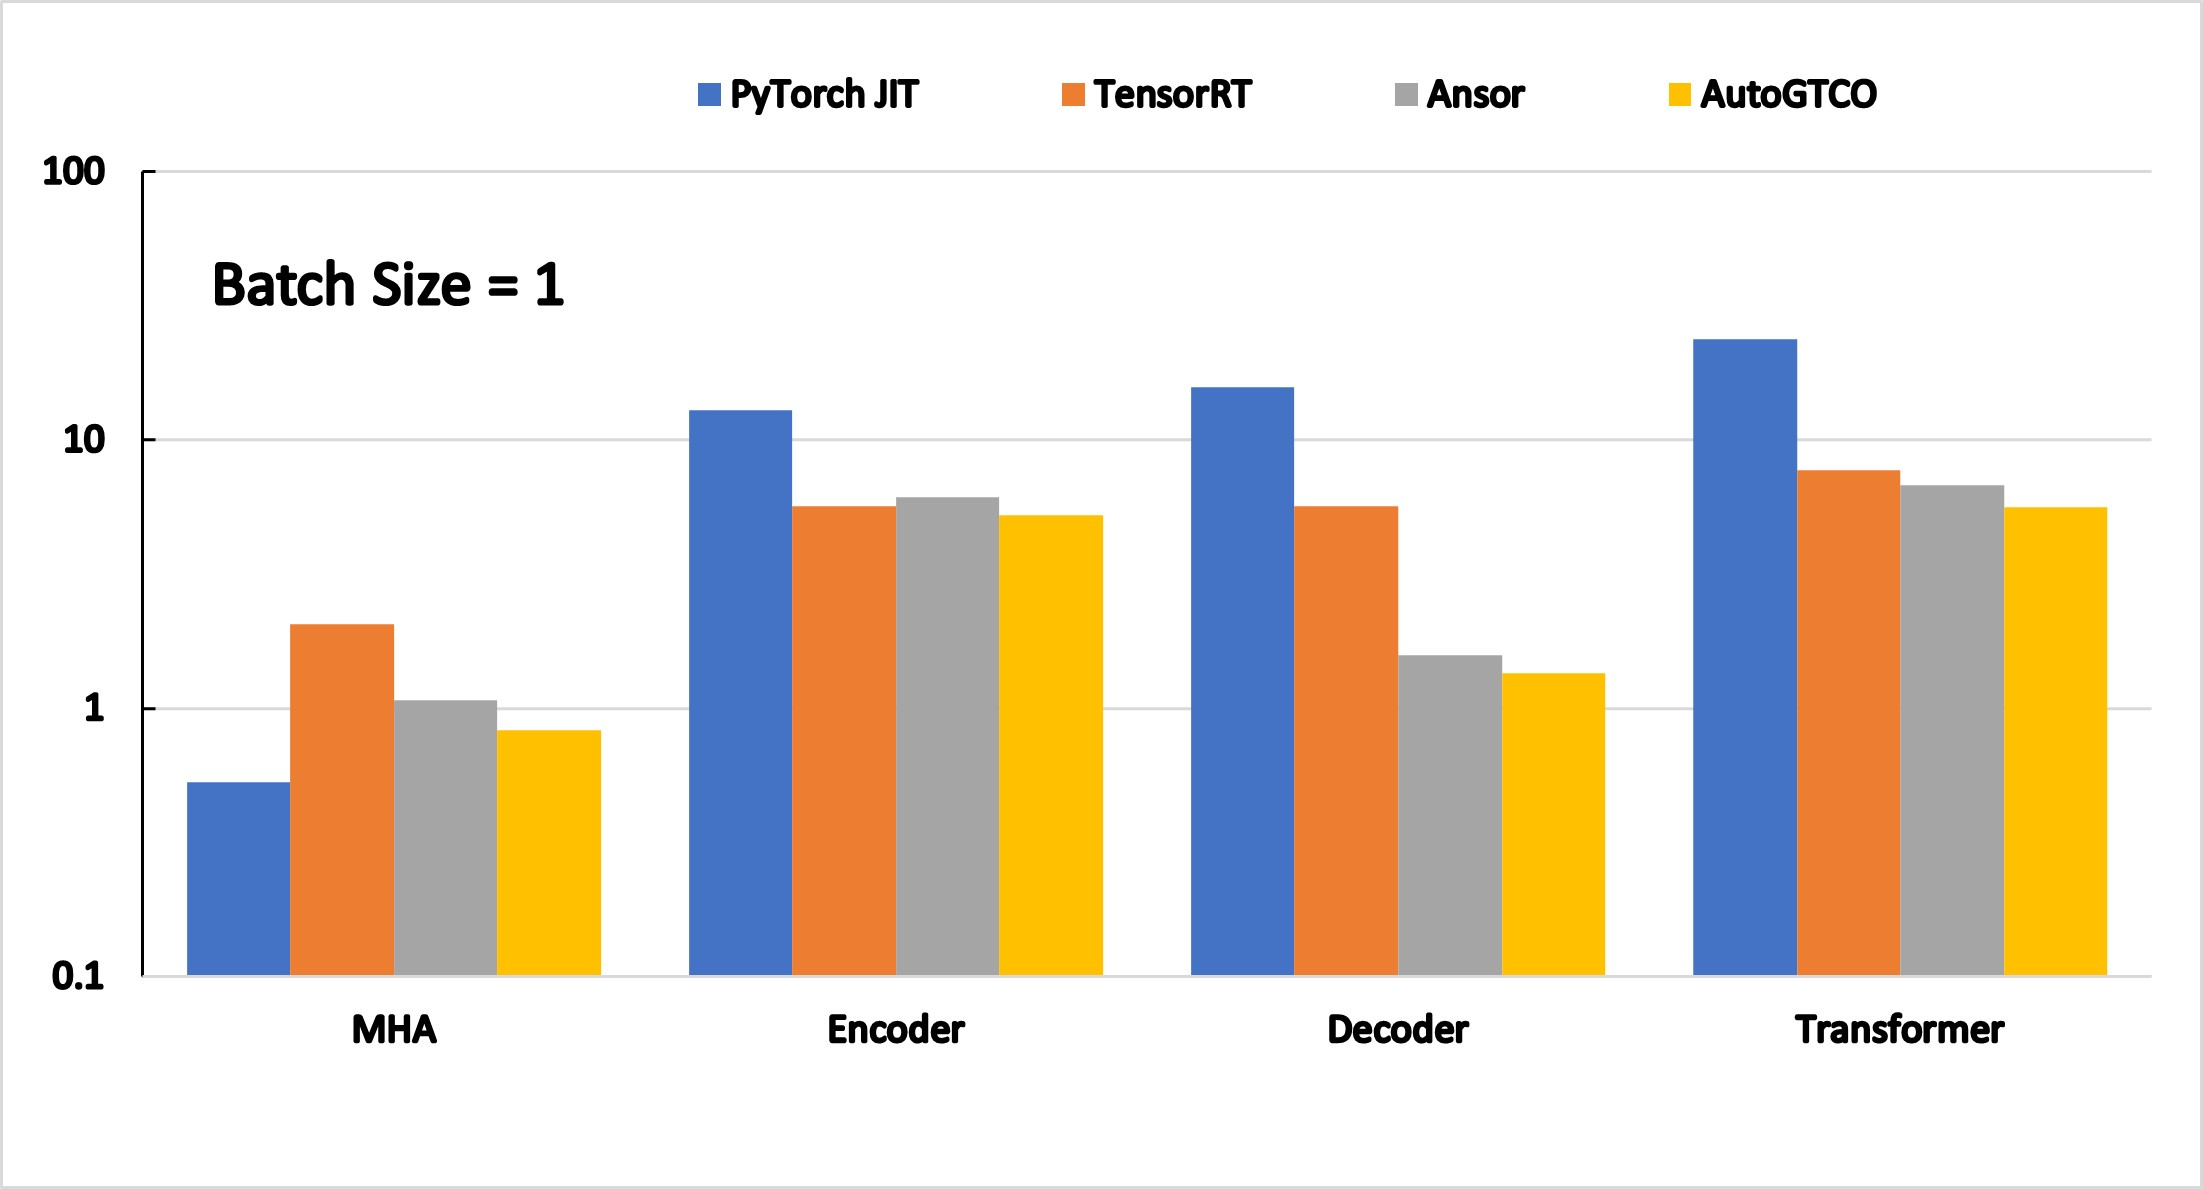
\includegraphics[height=4cm, width=6cm]{figs/fig8}
    \caption{xxx}
    \label{fig:fig8}
\end{figure}



\subsection{End-to-End Performance}
\textbf{Workloads.} We benchmark the end-to-end inference execution time of three image recognition models with transformers, which include DETR ResNet-50
for object detection, SETR ResNet-50 for semantic segmentation, and ViT for image classification. We report the results for batch size 1. Table xxx shows the number of encoders, the number of decoders, and the input shape of the tensor for each subgraph and network. \\
\textbf{Baselines and Configurations.} We include PyTorch JIT, TensorRT, and Ansor as baseline frameworks. Like the definition, we expect that
the end-to-end exeuction time they can achieve will be the sum of the latency of all subgraphs in a computation graph. We let both Ansor and AutoGTCD run 
auto-tuning 10000 measurement trails unless it converges to a stable value. The objective of subgraph scheduler is set to minimize the total execution time
of a transformer model and then generate efficient tensor programs for these subgraphs.\\
\textbf{Results.} Table xxx shows the results on a NVIDIA GeForce RTX 2080Ti GPU. In general, AutoGTCO surpasses all of the baseline frameworks expect for the ViT model. The reason for the decrease performance on ViT is that the input shape of ViT is small (224x224). After the partitioning of the input
image, each image is divided into smaller patches. As a result, the input shape of the tensor for encoder is also very small, which can not be well optimized by our methods, as shown and explained in the xxx. Compared with vendor-specific deep learning library TensorRT, AutoGTCO
has more advantages on uncommon shapes, because it is not easy to manually optimize for these cases in real-world scene.


% {\color{red} DETR:}

% Attention mechanisms in the transformer models are the key components which model relations between feature representations of different location of objects.
% %For the study 
% we choose ResNet-50-based DETR model with \textbf{6} encoder, \textbf{6} decoder layers and width \textbf{256}. 
% To be comparable in the number of paramters we choose a model with 6 encoder and 6 decoder layers of width 256 with 8 attention heads. \\

% {\color{red} SETR:}
% asada \\

% {\color{red} ViT:}
% ASDASD \\



% \textbf{Baselines.} asdada \\
% \textbf{Results.} asdasd \\
% \textbf{Abliation study.} asdasd \\



\label{sec:result}


\newpage
\begin{table*}[htbp]
    \caption{architecture of the model}
    \centering
    \scalebox{0.75}{
    \begin{tabular}{l|l|l|l|l|l|l|l|l|l|l}
    \hline
    model               & encoder & decoder & width & nhead & input shape           & patch & transformer input                                                                     & mha input                                                                                                            & encoder input          & decoder input                                                                             \\ 
    \hline
    \hline
    resnet50-based DETR & 6       & 6       & 256   & 8     & {[}1, 3, 800, 1333{]} & N/A   & \begin{tabular}[c]{@{}l@{}}src {[}1050,1, 256{]} \\ tgt {[}100,1, 256{]}\end{tabular} & \begin{tabular}[c]{@{}l@{}}query {[}1050, 1, 256{]}\\ key {[}1050, 1, 256{]}\\ value {[}1050, 1, 256{]}\end{tabular} & src {[}1050, 1, 256{]} & \begin{tabular}[c]{@{}l@{}}tgt {[}100, 1, 256{]}\\ memory {[}1050, 1, 256{]}\end{tabular} \\
    \hline
    SETR-Naive          & 24      & 1       & 1024  & 16    & {[}1, 3. 768, 768{]}  & 16    & \begin{tabular}[c]{@{}l@{}}src {[}2304,1, 1024{]} \\ tgt {[}2304, 1, 1024{]}\end{tabular} & \begin{tabular}[c]{@{}l@{}}query {[}2304, 1, 1024{]}\\ key {[}2304, 1, 1024{]} \\ value {[}2304, 1, 1024{]}\end{tabular} &   src {[}2304, 1, 1024{]}    &   {[}2304, 1, 1024{]}                                 \\
    \hline
    ViT-Base-16         & 12      & 0       & 768   & 12    & {[}1, 3, 224, 224{]}  & 16    & \begin{tabular}[c]{@{}l@{}}src {[}197, 1, 768{]} \\ tgt {[}197, 1, 768{]}\end{tabular}    & \begin{tabular}[c]{@{}l@{}}query {[}197, 1, 768{]}\\ key {[}197, 1, 768{]} \\ value {[}197, 1, 768{]}\end{tabular}  &     src {[}197, 1, 768{]}   &     N/A                                                    \\ 
    \hline
    \end{tabular}
    }
\end{table*} 


\begin{table*}[htbp]
    \caption{batch matrix multiplication and softmax in MHA}
    \centering
    \begin{tabular}{|l|l|l|l|l|l|l|l|}
    \hline
    layers (encoder) & GFLOPS & \#params & mAP  & PyTorch JIT & TensorRT & Ansor & Our method  \\ \hline
    3                & 81     & 37.4M    & 40.1 & 5.64        & 2.87     & 2.71  & 2.37        \\ \hline
    6                & 86     & 41.3M    & 40.6 & 11.45       & 5.65    & 6.13  & 5.25         \\ \hline
    12               & 95     & 49.2M    & 41.6 & 23.17       & 11.37    &  12.35     &  9.98            \\ \hline
    \end{tabular}
\end{table*}


% \begin{table*}[htbp]
%     \caption{dynamic programming for operator fusion on DETR}
%     \centering
%     \scalebox{0.75}{
%     \begin{tabular}{|l|l|l|l|l|l|l|l|}
%     \hline
%              & encoder & weights & decoder & weights & transformer & weights  & measurement trails \\ \hline
%     Ansor    &     9       &   (6 \times 7) (12 \times 2) &    13   & (6 \times 10) (18 \times 3)  &  22   &  (6 \times 17) (13 \times 2) (18 \times 1) (19 \times 2)                   &        10000            \\ \hline
%     AutoGTCO &              &                        &                      &                     &                          &                        &       8790             \\ \hline
%     \end{tabular}
%     }
% \end{table*}


\begin{table*}[htbp]
\caption{dp operator fusion}
\centering
\begin{tabular}{|l|l|l|l|l|l|l|l|}
\hline
         & n1 & weightEncoder                  & n2 & weightDecoder                   & n3 & weightTransformer                                         & measurement trails \\ \hline
Ansor    & 9  & {[}6 * 7{]} {[}12 * 2{]} & 13 & {[}6 * 10{]} {[}18 * 3{]} & 22 & {[}6 * 17{]} {[}13 * 2{]} {[}19 * 2{]} {[}18 * 1{]}  & 10000\\ \hline
AuToGTCO & 6   & {[}8 * 4{]} {[}10 * 2{]} & 11   &  {[}8 * 6{]} {[}20 * 5{]}  &  17  & {[}9 * 12{]} {[}20 * 3{]} {[}16 * 2{]}         & 8790            \\ \hline
\end{tabular}
\end{table*}


\begin{table*}[htbp]
    \caption{DETR Acceleration}
    \centering
    \begin{tabular}{|l|l|l|l|l|l|}
    \hline
                & MHA  & Encoder & Decoder & Transformer & Speedup \\ \hline
    PyTorch JIT & 0.53 & 12.96   & 15.75   & 23.67       & -   \\ \hline
    TensorRT    & 2.05 & 5.65    & 5.65    & 7.73        & 1.00    \\ \hline
    Ansor       & 1.07 & 6.13    & 1.58    & 6.78        & 1.12x   \\ \hline
    AutoGTCO    & 0.83 & 5.25    & 1.35    & 5.60        & 1.27x   \\ \hline
    \end{tabular}
\end{table*}


\begin{table}[htbp]
    \caption{image recognition with transformers acceleration}
    \centering
    \scalebox{0.85}{
    \begin{tabular}{|l|l|l|l|l|}
    \hline
                   & PyTorch JIT & TensorRT & Ansor & AutoGTCO \\ \hline
    DETR-ResNet-50 & 23.67       &  7.73    & 6.78  & 5.60     \\ \hline
    SETR-Naive     & 68.26       &  33.71   &       &          \\ \hline
    ViT-Base-16x16 & 24.92       &  5.87    & 8.57  & 8.43     \\ \hline
    \end{tabular}
    }
\end{table}